\section{Wechselkurse}

\subsection{Nominaler Wechselkurs}
Erhöht sich die inländische Geldmenge im Vergleich zur ausländischen, dann steigt der nominale Wechselkurs. Dies ist eine Abwertung der inländischen Währung. Umgekehrt ist eine Erhöhung der ausländischen Geldmenge eine Aufwertung der inländischen Währung. 
\begin{equation*}
 e\quad\text{(nominaler Wechselkurs)} = \frac{\text{inländische  Währung}}{\text{ausländische Währung}}
\end{equation*}

\subsection{Realer Wechselkurs}
Bei den realen Wechselkursen werden die unterschiedlichen Preisniveaus im Inland und Ausland berücksichtigt.
\begin{equation*}
	r\quad \text{(realer Wechselkurs)} = \frac{e \cdot p^{*}\quad \text{(Preis Güterkorb  im Ausland in  ausländischer  Währung)}}{p\quad \text{(Preis\ Güterkorb im Inland in inländischer Währung})}
\end{equation*}
\begin{description}
	\item[p*] Ausländisches Preisniveau (Inflation im Ausland)
	\item[p] Inländisches Preisniveau (Inflation im Inland)
\end{description}
\begin{itemize}
	\item e: ändert sehr schnell (täglich)
	\item p: ändert sehr langsam (Monate bis Jahre)
\end{itemize}
Wenn r > 1 ist der Güterkorb im Ausland teurer.

\subsubsection{Kurzfristiger/Langfristiger Effekt}
\begin{multicols}{2}
	\textbf{kurzfristig}\\
	Bei einer Ausweitung der inländischen Geldmenge reagiert der nominale Wechselkurs sofort, das inländische Preisniveau kurzfristig aber nicht.\\
	Für die Exportindustrie ist es gut, da die Produkte für das Ausland günstiger werden.\\
	\vspace{\baselineskip}
	\textbf{langfristig}\\
	Eine Ausweitung der inländische Geldmenge führt zu keiner Veränderung des realen Wechselkurses, da sich das inländische Preisniveau anpasst.\\
	\vspace{\baselineskip}
	\textbf{Bsp.: Geldpolitik der Bank of Japan}
	Die Bank of Japan weitet ihre Geldmenge seit einigen Jahren kräftig aus.\\
	\begin{description}
		\item[kurzfristig:] Toyota wird grösster Authersteller der Welt, weil der Preis international gesunken ist
		\item[langfristig:] Effekt bricht zusammen
	\end{description}
	\vfill\null
	\columnbreak
	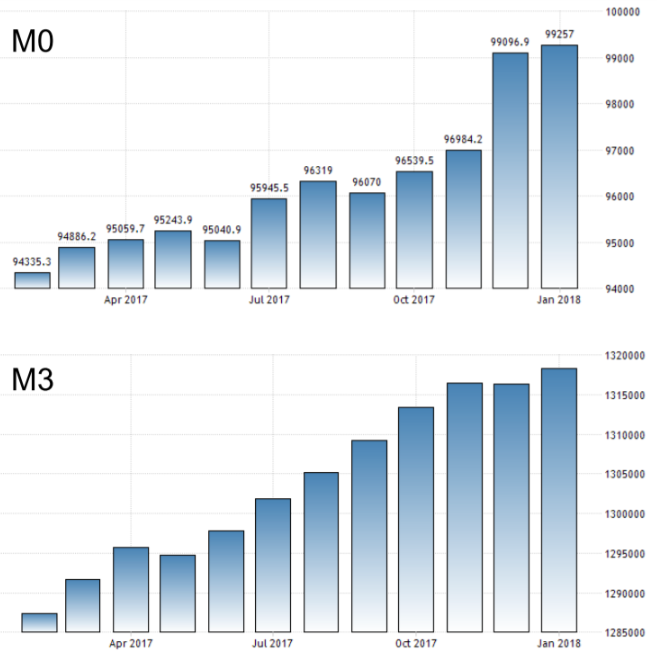
\includegraphics[width=0.8\linewidth]{images/bankofjapan.png}
\end{multicols}

\subsection{Fixe Wechselkurssysteme}
\begin{itemize}
	\item Ankoppelung der eigenen Währung an eine Fremdwährung (Leitwährung)
	\item Vorteile:
	\begin{itemize}
		\item Berechenbarkeit der Wechselkurse für die Export-/Importindustrie
		\item Anbindung der eigenen Geldpolitik an die stabilere Geldpolitik des Landes der Leitwährung
	\end{itemize}
	\item Nachteile:
	\begin{itemize}
		\item Aufgabe einer eigenständigen Geldpolitik zur Konjunktursteuerung
	\end{itemize}
\end{itemize}
\clearpage

\textbf{EWS (Europäisches Währungssystem)}\\
\begin{itemize}
	\item bis Anfang der 1970er Jahre Bretton-Woods-System (Leitwährung US-Dollar)
	\item 1979 EWS mit D-Mark als Leitwährung eingeführt (Vereinfachung der Handelsbeziehungen; Vermeidung eines $"$Währungskrieges$"$ zur Unterstützung der nationalen Exportindustrien)
	\item Wechselkurs liess man nur innerhalb enger, vorher vereinbarten Bandbreiten schwanken
	\item Probleme: 
	\begin{itemize}
		\item zu Beginn grosse Inflationsunterschiede (z.B. Italien und Deutschland); Fixierung des nominalen Wechselkurses $\rightarrow$ massive Auswirkungen auf realen Wechselkurs
		\item fixe Wechselkurse führen zwangsläufig dazu, dass Mitgliedsländer die Geldpolitik des Leitwährungslandes imitieren müssen; diese kann im Widerspruch zur konjunkturellen Entwicklung eines Mitgliedlandes stehen
		\item Zwei Formen von Inkonsistenzen, welche Spekulanten nutzen können:
		\begin{itemize}
			\item zwischen Konjunkturlage und Geldpolitik (Fall England)
			\item Beeinträchtigung der Wettbewerbsfähigkeit bei grossen Inflationsunterschieden durch reale Aufwertung der inländischen Währung (Fall Italien)
		\end{itemize}
		\item Beide Fälle zeigen auf, dass "falsche Wechselkurse" langfristig nicht verteidigt werden können!
	\end{itemize}
\end{itemize}
\begin{multicols}{2}
	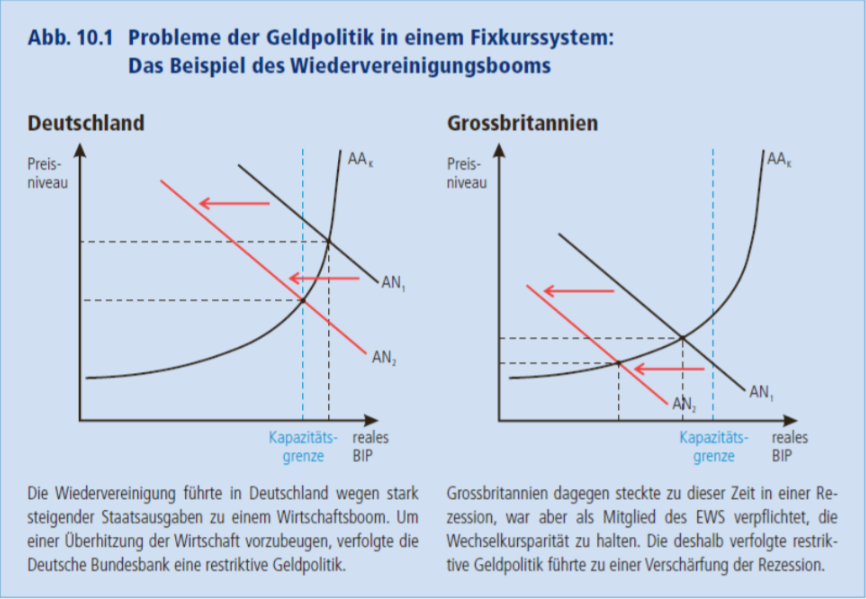
\includegraphics[width=\linewidth]{images/fixkurs.png}
	Devisenspekulant: mit Pfund D-Mark kaufen $\rightarrow$ nach Austritt: mit D-mark Pfund kaufen
	\vfill\null
	\columnbreak
	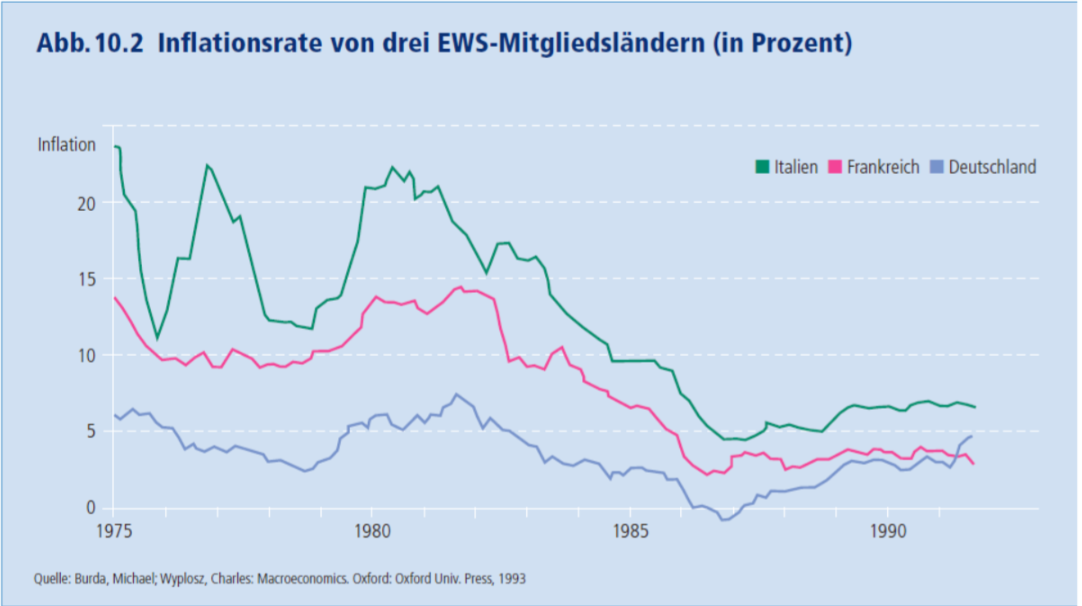
\includegraphics[width=0.7\linewidth]{images/inflationskonvergenz.png}
	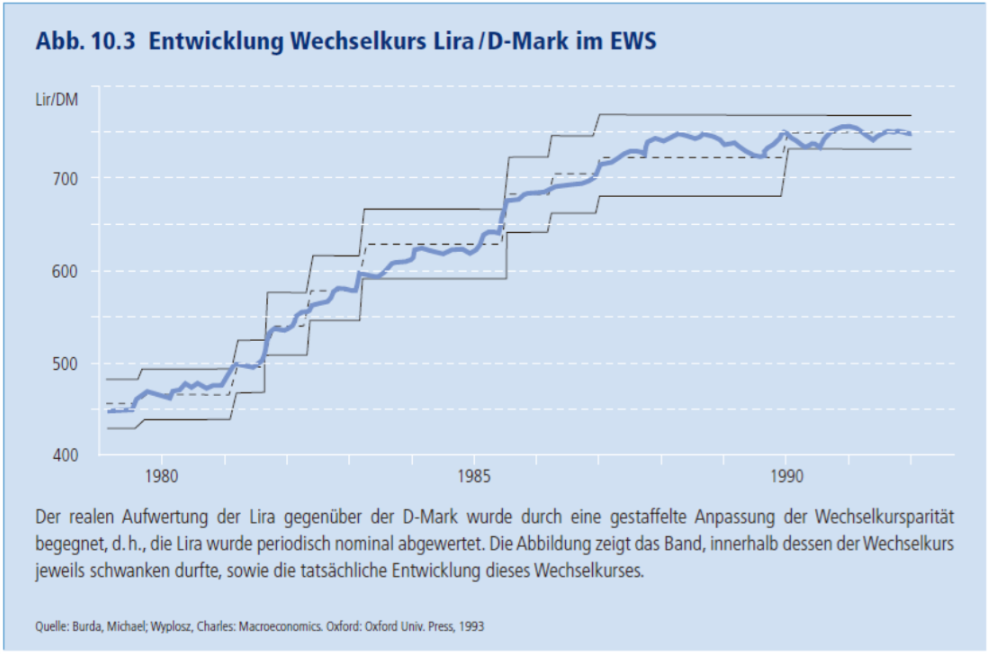
\includegraphics[width=0.7\linewidth]{images/inflationskonvergenz2.png}
	Devisenspekulant: mit Lira D-Mark kaufen $\rightarrow$ nach Lira-Abwertung: mit D-Mark Lira kaufen
\end{multicols}

\subsection{Währungsunion}
\textbf{Unterschiede fixes Wechselkurssystem und Währungsunion}\\
\begin{itemize}
	\item In einem fixen Wechselkurssystem sind die Kurse nicht für alle Zeiten fixiert. Jedes Land kann aus dem System aussteigen.
	\item In der Währungsunion sind die nominalen Wechselkurse fixiert durch eine Zentralbank, nicht durch nationale Geldpolitiken.
\end{itemize}
\textbf{Vorteile:}\\
\begin{itemize}
	\item Kein Wechselkursrisiko und keine Transaktionskosten bei Währungstausch
	\item Erhöhung der Preistransparenz, da Güterkorbpreise direkt verglichen werden können.
	\item Länder in der Währungsunion sollten in konjunktureller Entwicklung ähnlich sein, ansonsten drohen durch Geldpolitik $"$asymmetrische Schocks$"$.
	\begin{itemize}
		\item Falls trotzdem Unterschiede bestehen, sollten diese durch:
		\begin{itemize}
			\item{\makebox[5cm]{flexible Löhne \& Preise,\hfill}} EU: können nur steigen
			\item{\makebox[5cm]{mobile Arbeitskräfte und\hfill}} EU: Sprachbarriere 
			\item{\makebox[5cm]{ausgleichende Fiskalströme\hfill}} EU: "Peanuts"
		\end{itemize}
		 aufgefangen werden; anstatt durch die nationale Geldpolitik.
	\end{itemize}
\end{itemize}
\vspace{\baselineskip}
\begin{multicols}{2}
\textbf{EWU (Europäische Währungsunion)}\\
Anfangs der 90er Jahre legte der Vertrag von Maastricht den Prozess der Weiterentwicklung der EG (Europäischen Gemeinschaft) zur EWU (Einführung Euro 1999) fest (mehr zur EWU in Kap. \ref{sec:EWU}).
\vfill\null
\columnbreak
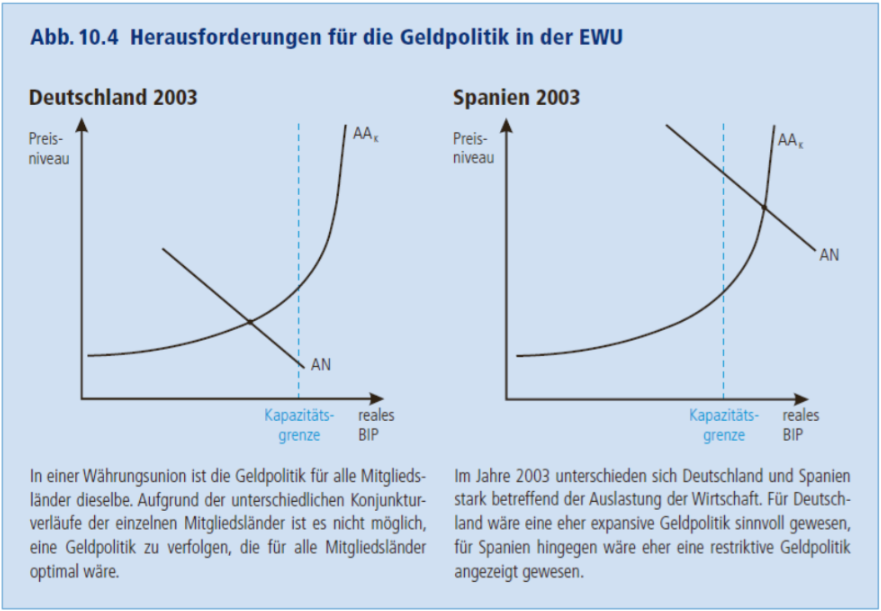
\includegraphics[width=\linewidth]{images/ewu.png}
\end{multicols}


\begin{itemize}
	\item \textbf{Frühe Kritik:}
	\begin{itemize}
		\item Mitgliedsländer sind konjunkturell trotz Erfüllung der Konvergenzkriterien zu unterschiedlich
		\item Anpassungsmechanismen sind nur schwach ausgebaut:
		\begin{itemize}
			\item wenig flexible Löhne, stark regulierte Arbeitsmärkte
			\item wenig mobile Arbeitskräfte wegen Sprachbarriere (im Vergleich zur USA)
			\item geringe ausgleichende Fiskalströme, da das zentral verwaltete Budget nicht gross genug ist (aktuell ca. 125 Mia. Euro jährlich)
		\end{itemize}
	\end{itemize}
	\item Einführung der EWU trotz Vorbehalten aus folgenden Gründen:
	\begin{itemize}
		\item EU sowie EWU muss als (friedens-)politisches und nicht ökonomisches Projekt betrachtet werden
		\item Grundidee besteht in weiterführender Integration der europäischen Staaten zu einem "Europa"
	\end{itemize}
\end{itemize}
\begin{multicols}{2}
	\begin{itemize}
		\item \textbf{Eurokrise:}
		\begin{itemize}
			\item Seit 2013 kämpft die Eurozone mit der schwersten Krise seit Gründung
			\item wegen massiver Überschuldung Griechenlands stieg Besorgnis über Staatsverschuldung europäischer Staaten an
			\item Finanzmärkte begannen an Rückzahlungsfähigkeit der PIGS-Staaten zu zweifeln
			\item seit Einführung des Euros bauten sich gewaltige makroökonomische Ungleichgewichte auf
			\item Anleger gingen davon aus, dass bei zentraler Geldpolitik das Risiko von staatlichen Anleihen in allen Mitgliedsstaaten gleich hoch ist
			\item für PIGS-Staaten war dies eine "billige" Möglichkeit der Staatsverschuldung
			\item dies führte anfangs zu einem Wirtschaftsboom in diesen Ländern, weil tiefe Zinsen die Investitionen der Unternehmen, den Konsum der Haushalte und des Staates stimulierten
			\item langfristig führte dies aber zu zwei fatalen Ungleichgewichten:
			\begin{itemize}
				\item Reduktion der Wettbewerbsfähigkeit der PIGS-Staaten (realer Wechselkurs sinkt)
				\item Ausufernde Staatsverschuldung
			\end{itemize}
		\end{itemize}
	\end{itemize}
	\vfill\null
	\columnbreak
	\includegraphics[width=\linewidth]{images/eurokrise.jpg}
	\vspace{\baselineskip}
	Verlust der Wettbewerbsfähigkeit:
	$r\downarrow = \frac{e \cdot p^*}{p\uparrow}$
	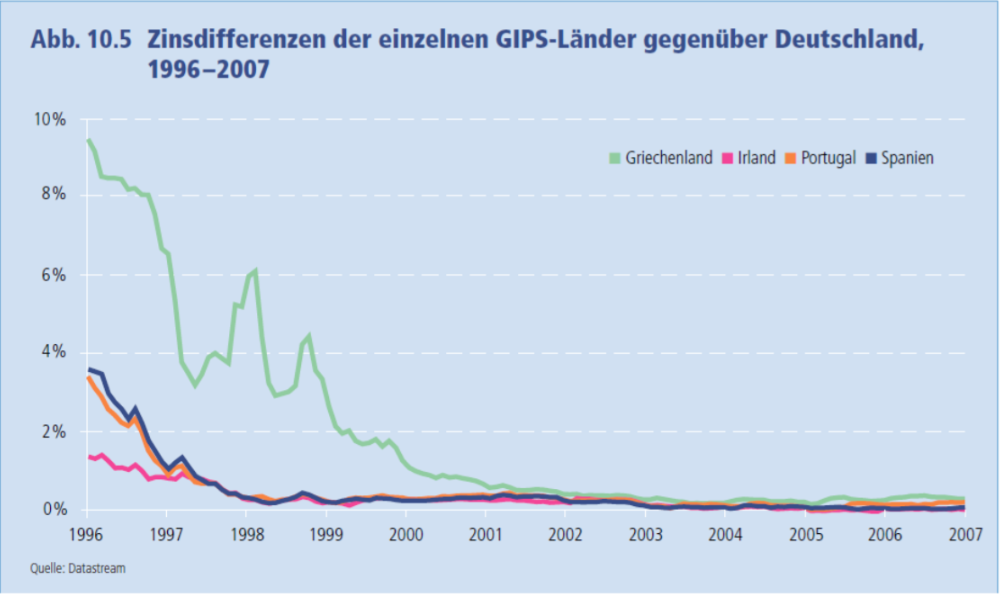
\includegraphics[width=\linewidth]{images/pigs.png}
	\vfill\null
\end{multicols}
\clearpage
\pagebreak